\documentclass[a4paper]{article}
\usepackage{float}
\usepackage[spanish,es-tabla]{babel}
\usepackage[T1]{fontenc}
\usepackage[spanish]{babel}
\usepackage{graphicx} 
\usepackage[utf8]{inputenc}
\usepackage{amsmath}
\usepackage{longtable}
\usepackage{graphicx}
\usepackage[colorinlistoftodos]{todonotes}
\usepackage[letterpaper,top=2.5cm,bottom=2.5cm,left=2cm,right=2cm,marginparwidth=2.5cm]{geometry}
\renewcommand{\baselinestretch}{1.25}


\title{Informe Física 6}
\author{Danny Córdova, Edwin Dávila}
\date{28 de Marzo del 2023}



\begin{document}

\maketitle

\section{Introducción}

En la presente práctica se estudiará la conservación de la energía. Siendo más precisos, se estudiará la energía mecánica porque para estudiar la conservación de la energía y hacer que se cumpla el principio de conservación se debería ser capaz de tener en cuenta a todas las fuerzas que están actuando sobre el sistema en estudio, lo cual sale de las capacidades del experimento. En este experimento se toma en cuenta a la energía potencial elástica, energía potencial gravitatoria, fricción con la superficie y energía cinética. Como objetivo general de la práctica se tiene el demostrar que la energía final total del sistema es menor a la energía inicial.

\section{Metodología experimental}
Las unidades usadas en este experimento son las del SI. Las incertidumbres de los instrumentos de medida son:

\begin{table}[H]
    \centering
    \begin{tabular}{|c|c|}
    \hline
        Regla  & $\pm 1 mm$ \\ \hline
        Cronómetro digital  & $\pm 0,01 ms$ \\ \hline
    \end{tabular}
    \caption{Incertidumbre de los instrumentos de medida}
    \label{Incertidumbre de los instrumentos de medida}
\end{table}

El siguiente diagrama esboza como se realizó el experimento:
\begin{figure} [H]
    \centering
    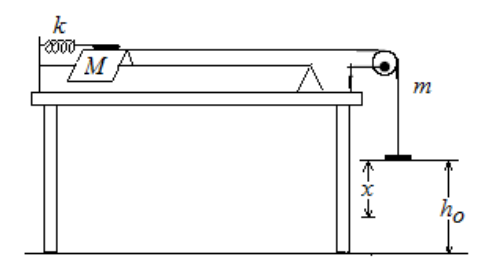
\includegraphics{Diagrama Lab 6.png}
    \caption{Diagrama del experimento}
    \label{fig:my_label}
\end{figure}

Las medidas que se mantienen constantes son:

\begin{table}[H]
    \centering
    \begin{tabular}{|c|c|c|c|}
    \hline
        (x) natural del resorte & 12.6 $\pm$ 0,1 cm & (h) del móvil & 104 $\pm$ 0,1 cm   \\ \hline
       ($h_i$) del portamasas & 68.7 $\pm$ 0,1 cm & (m) del móvil & 104 $\pm$ 1g \\ \hline 
       (m) del portamasas & 50 $\pm$ g & (x) en 1 & 16.5 $\pm$ 0.1 cm \\ \hline
       (h) en 1 & 64.1 $\pm$ 0.1 cm & (x) en 2 & 36.5 $\pm$ 0.1 cm \\ \hline
       (h) en 2 & 36.5 $\pm$ 0.1 cm & & \\ \hline
             
    \end{tabular}
    \caption{Medidas constantes}
    \label{Medidas constante}
\end{table}

Las variables directas que se miden en este experimento son:
\begin{enumerate}
  \item Velocidad instantánea en el obturador (v).
  \item Elongación del resorte (x).
  \item Altura de la base al portamasas (h).
\end{enumerate}

Las variables indirectas que se calculan a partir de la información obtenida son:
\begin{enumerate}
  \item Constante de elongación del resorte (k).
  \item Energía potencial gravitatoria ($U$).
  \item Energía potencial elástica ($E_p$)
  \item Energía cinética (K)
\end{enumerate}

Las fórmulas usadas en este experimento son:

\begin{equation}
    y=mx+b
\end{equation}
esta fórmula representa la ecuación de una recta y sirve para hacer la regresión lineal. Aquí x es la variable independiente y y la variable dependiente. 

\begin{equation}
   m=\frac{\sum x_i*y_i-\frac{1}{n}\sum x_i \sum y_i}{\sum x_i^2-\frac{1}{n}(\sum x_i)^2} 
\end{equation}
donde m es la pendiente de la regresión lineal y n es el número de datos.

\begin{equation}
    b=\frac{\sum y_i}{n}-m\frac{\sum x_i}{n}
\end{equation}
donde b es el corte en el eje y de la regresión lineal.

\begin{equation}
    E_p=\frac{1}{2}k\Delta x^2
\end{equation}
donde $E_p$ es la energía potencial elástica, k la constante de elongación y $\Delta x$ el cambio en la elongación del resorte. 

\begin{equation}
    U=mgh
\end{equation}
donde U es la energía potencial gravitatoria, m la masa del objeto, g la gravedad y h la altura a la que se encuentra el objeto en relación al suelo.

\begin{equation}
    K=\frac{1}{2}mv^2
\end{equation}
donde K es la energía cinética y v la velocidad a la que se mueve el objeto. 

\begin{equation}
    W_{01}=K_0+K_1
\end{equation}
donde W es el trabajo en un intervalo de tiempo y $K_0$ y $K_1$ la energía cinética en los extremos de ese intervalo. Este es el principio de Trabajo-Energía.

\begin{equation}
    f_{fric}=-\mu N
\end{equation}
    donde $f_{fric}$ es la fuerza de fricción, $\mu$ es el coeficiente de fricción y N la fuerza normal

\begin{equation}
    \Delta E_{mec}=\Delta K+\Delta U+\Delta E_p=-f_{fric}x
\end{equation}
donde $\Delta E_{mec}$ es la variación de la energía mecánica

\section{Resultados y observaciones}
Con la fórmulas (4), (5) y (6) calculamos la energía total, siendo la suma de energía cinética y potencial en cada punto, en Anexos se tiene una vista detallada de los datos.

\begin{table}[!ht]
    \centering
    \begin{tabular}{|c|c|c|c|c|c|}
    \hline
        ~ & 50 & 70 & 90 & 100 & 110  \\ \hline
        Energía total en (0) & 336,694 & 471,371 & 606,049 & 673,387 & 740,726  \\ \hline
        Energía total en (1) & 323,130 & 461,271 & 604,784 & 672,653 & 744,124  \\ \hline
        Energía total en (2) & 225,975 & 330,342 & 446,757 & 509,755 & 564,966  \\ \hline
        Energía total en (3) & 258,041 & 281,928 & 267,534 & 252,319 & 232,431  \\ \hline
    \end{tabular}
    \caption{Energía total en cada punto}
    \label{Energía total en cada punto}
\end{table}

A partir de esta y considerando la energía inicial, calculamos el porcentaje de energía perdida usando:

\[\% E_{perdida} = \frac{\Delta E}{E_i}100\%\]

\begin{table}[!ht]
    \centering
    \begin{tabular}{|c|c|c|c|c|c|}
    \hline
        ~ & 50 & 70 & 90 & 100 & 110  \\ \hline
        Energía perdida 1 & 4,028\% & 2,142\% & 0,208\% & 0,109\% & -0,459\%  \\ \hline
        Energía perdida 2 & 66,43\% & 29,90\% & 26,27\% & 24,29\% & 23,72\%  \\ \hline
        Energía perdida 3 & 61,68\% & 40,17\% & 55,83\% & 62,50\% & 68,58\%  \\ \hline
    \end{tabular}
    \caption{Porcentaje de energía perdida}
    \label{Porcentaje de energía perdida}
\end{table}

Para finalizar calculamos el coeficiente de fricción de la pista, usando (9) y despejando $\mu$ obtenemos:

\[ \mu = - \frac{\Delta K+\Delta U+\Delta E_p}{Nd}\]

\begin{table}[H]
\centering
    \begin{tabular}{|c|c|c|c|c|c|}
    \hline
        & 50 & 70 & 90 & 100 & 110 \\ \hline
        $\mu$ &  0.4051 & 0.5160 & 0.5829 & 0.5987 & 0.64312 \\ \hline
    \end{tabular}
    \caption{Coeficiente de fricción dinámico por cada peso}
    \label{Coeficiente de fricción dinámico}
\end{table}

\section{Conclusiones}

En la presente práctica se pudo comprobar la conservación de la energía al analizar las energías resultantes en cada punto del movimiento con las diferentes masas. Solo existe un error en el cálculo de la energía de la masa de 110 g en la posición inicial y en el sensor 1, le energía en el sensor 1 es mayor que la energía en la posición inicial y probablemente este error se dio porque al momento de soltar el móvil se aplicó una fuerza involuntariamente que le dio un impacto extra al móvil. Por otro lado, se cumplió el objetivo de esta práctica satisfactoriamente. 

\section{Anexos}

\begin{table}[H]
    \centering
    \begin{tabular}{|c|c|}
    \hline
        Peso (kg) & Elongación  \\ \hline
        0 & 0,101  \\ \hline
        0,48867 & 0,303  \\ \hline
        0,586404 & 0,358  \\ \hline
        0,684138 & 0,411  \\ \hline
        0,781872 & 0,456  \\ \hline
        0,879606 & 0,512  \\ \hline
        0,97734 & 0,561  \\ \hline
        1,075074 & 0,609  \\ \hline
        1,172808 & 0,659  \\ \hline
        1,270542 & 0,705  \\ \hline
        1,368276 & 0,758  \\ \hline
    \end{tabular}
    \caption{Elongación del resorte a diferentes pesos}
    \label{Elongación del resorte a diferentes pesos}
\end{table}


\begin{table}[H]
    \centering
    \begin{tabular}{|c|c|c|c|c|c|}
    \hline
        Inicial & 50 & 70 & 90 & 100 & 110  \\ \hline
        Potencial gravitatoria & 336,694 & 471,371 & 606,049 & 673,387 & 740,726  \\ \hline
        Potencial Elástica & 0,000 & 0,000 & 0,000 & 0,000 & 0,000  \\ \hline
        Total Ep & 336,694 & 471,371 & 606,049 & 673,387 & 740,726  \\ \hline
        Cinética & 0,000 & 0,000 & 0,000 & 0,000 & 0,000  \\ \hline
        Total E & 336,694 & 471,371 & 606,049 & 673,387 & 740,726  \\ \hline
    \end{tabular}
\caption{Datos posición inicial del cuerpo (0)}
\label{Datos posición inicial del cuerpo}
\end{table}

\begin{table}[H]
    \centering
    \begin{tabular}{|c|c|c|c|c|c|}
    \hline
        En (1) & 50 & 70 & 90 & 100 & 110  \\ \hline
        Potencial gravitatoria & 313,237 & 438,532 & 563,827 & 626,475 & 689,122  \\ \hline
        Potencial Elástica & 0,002 & 0,002 & 0,002 & 0,002 & 0,002  \\ \hline
        Total Ep & 313,239 & 438,534 & 563,829 & 626,476 & 689,124  \\ \hline
        Cinética & 9,891 & 22,737 & 40,955 & 46,176 & 55,000  \\ \hline
        Total E & 323,130 & 461,271 & 604,784 & 672,653 & 744,124  \\ \hline
    \end{tabular}
    \caption{Datos en sensor 1}
    \label{Datos en sensor 1}
\end{table}

\begin{table}[H]
    \centering
    \begin{tabular}{|c|c|c|c|c|c|}
    \hline
        En (2) & 50 & 70 & 90 & 100 & 110  \\ \hline
        Potencial gravitatoria & 214,526 & 300,337 & 386,147 & 429,052 & 471,957  \\ \hline
        Potencial Elástica & 0,058 & 0,058 & 0,058 & 0,058 & 0,058  \\ \hline
        Total Ep & 214,584 & 300,395 & 386,205 & 429,110 & 472,016  \\ \hline
        Cinética & 11,391 & 29,947 & 60,552 & 80,645 & 92,950  \\ \hline
        Total E & 225,975 & 330,342 & 446,757 & 509,755 & 564,966  \\ \hline
    \end{tabular}
    \caption{Datos en sensor 2}
    \label{Datos en sensor 2}
\end{table}

\begin{table}[H]
    \centering
    \begin{tabular}{|c|c|c|c|c|c|}
    \hline
        Punto de equilibrio & 50 & 70 & 90 & 100 & 110  \\ \hline
        Potencial gravitatoria & 258,018 & 281,865 & 267,400 & 252,154 & 232,216  \\ \hline
        Potencial Elástica & 0,023 & 0,063 & 0,134 & 0,166 & 0,215  \\ \hline
        Total Ep & 258,041 & 281,928 & 267,534 & 252,319 & 232,431  \\ \hline
        Cinética & 0,000 & 0,000 & 0,000 & 0,000 & 0,000  \\ \hline
        Total E & 258,041 & 281,928 & 267,534 & 252,319 & 232,431  \\ \hline
    \end{tabular}
    \caption{Datos en punto de equilibrio (3)}
    \label{Datos en punto de equilibrio}
\end{table}

\begin{table}[H]
    \centering
    \begin{tabular}{|c|c|c|c|c|c|}
    \hline
        Masas & 50 & 70 & 90 & 100 & 110  \\ \hline
        $\Delta K$ & 11.391 & 29.947 & 60.552 & 80.645 & 92.950  \\ \hline
        $\Delta U$ & -122.16 & -171.04 & -219.90 & -244.34 & -268.77  \\ \hline
        $\Delta E_p$ & 0.058 & 0.058 & 0.058 & 0.058 & 0.058  \\ \hline
        
    \end{tabular}
    \caption{Variaciones de energía}
    \label{Variaciones de energía}
\end{table}

\end{document}